\documentclass{beamer}
\usepackage{tikz}
%\usetikzlibrary{positioning}
\usetikzlibrary{trees,shapes.geometric, positioning, calc}

\tikzstyle{state} = [circle, inner sep=2pt, radius =20pt, text centered, draw=black, fill=blue!50]
\tikzstyle{myarrow} = [->, >=latex]


\tikzstyle{point} = [circle, inner sep=0pt, minimum size =1pt,  fill=black]
\tikzstyle{process} = [rectangle, text centered, inner ysep=8pt,   path picture={ \draw[black,fill=\entryfill] (current bounding box.north) ++(0,-1pt)  circle (1pt) ++(0,-1pt) -- +(0,-2pt); \draw [black,fill=\exitfill] (current bounding box.south) ++(0,1pt) circle (1pt) ++(0,1pt) -- +(0,2pt); \draw[black,fill=blue!20]  ($(current bounding box.south west) + (0,4pt)$)  rectangle  ($(current bounding box.north east) - (0,4pt)$);  }]

\tikzstyle{io} = [rectangle, rounded corners, text centered, inner ysep=5pt,   path picture={ \draw[black] (current bounding box.north) ++(0,-1pt)  circle (1pt) -- ++(0,-3pt); \fill [black] (current bounding box.south) ++(0,1pt) circle (1pt); \draw[black,fill=green!20]  ($(current bounding box.south west) + (0,2pt)$)  rectangle  ($(current bounding box.north east) - (0,4pt)$);  }]

\tikzstyle{decision} = [diamond, aspect=2,  text centered,  inner ysep=5pt, path picture={ \draw[black,fill=\entryfill] (current bounding box.north)  ++(0,-1pt) circle (1pt) ++(0,-1pt) -- +(0,-2pt); \draw [black,fill=\exitfill] ($(current bounding box.south) +(0,1pt)$) circle (1pt) ++(0,1pt)  -- +(0,2pt); \draw[black ,fill=red!30]  (current bounding box.west)  -- ($(current bounding box.south) + (0,4pt)$) -- (current bounding box.east) -- ($(current bounding box.north) - (0,4pt)$) -- cycle;  }]

\tikzstyle{stop} = [circle,  text centered,  inner sep=4pt,  path picture={ \draw[black] (current bounding box.north)  -- +(0,-3pt); \draw[black,thick,fill=red ]  (current bounding box.center) let \p1 = ($(current bounding box.north) - (current bounding box.center) - (0,3pt)$) in  circle ({veclen(\x1,\y1)});}]
\tikzstyle{start} = [rectangle, rounded corners,  text centered, draw=black, fill=green]


\begin{document}
\begin{minipage}{.45\textwidth}
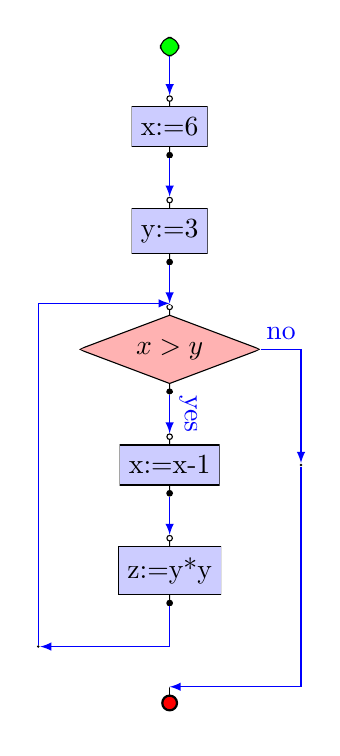
\begin{tikzpicture}[node distance = 2cm]

\def\entryfill{white}
\def\exitfill{black}
\tikzstyle{myarrow} = [->, blue, >=latex]

\matrix[row sep =5mm,column sep=5mm]{
 &\node(vert1)[start]{}; &\\
 &\node(vert9)[process]{x:=6}; &\\
 &\node(vert8)[process]{y:=3}; &\\
 &\node(vert5)[decision]{$x>y$}; &\\
 &\node(vert4)[process]{x:=x-1}; &\node(vert7)[point]{};\\
 &\node(vert3)[process]{z:=y*y}; &\\
\node(vert6)[point]{}; & &\\
 &\node(vert2)[stop]{}; &\\
};

\draw [myarrow]  (vert9.south) -- (vert8.north);
\draw [myarrow]  (vert4.south) -- (vert3.north);
\draw [myarrow]  (vert3) |- (vert6);
\draw [myarrow]  (vert6)  |-  (vert5.north);
\draw [myarrow]  (vert5.south)  -- node[sloped,above]{yes}  (vert4.north);
\draw [myarrow]  (vert5.east)  -| node[sloped,above, near start]{no}  (vert7.north);
\draw [myarrow]  (vert8.south) -- (vert5.north);
\draw [myarrow]  (vert1.south) -- (vert9.north);
\draw [myarrow]  (vert7.south) |- (vert2.north);
\end{tikzpicture}
\end{minipage}
\begin{minipage}{.45\textwidth}
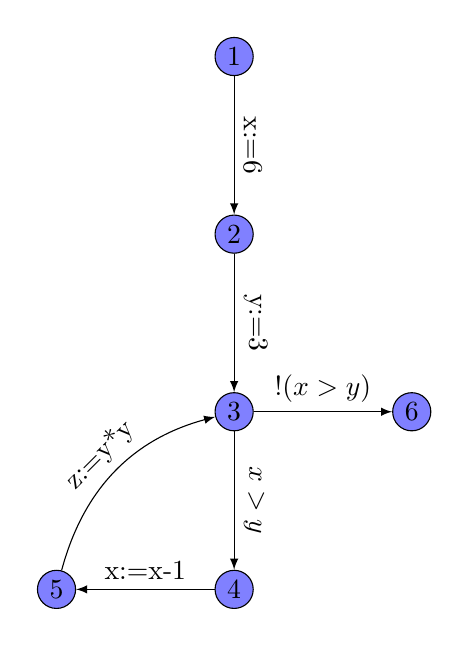
\begin{tikzpicture}[node distance = 2cm]
\matrix[row sep =5em,column sep=5em]{
 &\node(vert9)[state]{1}; &\\
 &\node(vert8)[state]{2}; &\\
 &\node(vert5)[state]{3}; &\node(vert2)[state]{6};\\
 \node(vert3)[state]{5}; &\node(vert4)[state]{4}; &\\
};
\draw [myarrow]  (vert9)  --  node[sloped, above]{x:=6} (vert8);
\draw [myarrow]  (vert8)  --  node[sloped, above]{y:=3} (vert5);
\draw [myarrow]  (vert5)  -- node[sloped,above]{$x>y$}  (vert4);
\draw [myarrow]  (vert4)  --  node[sloped, above]{x:=x-1} (vert3);
\draw [myarrow]  (vert3) edge[bend left]  node[sloped, above]{z:=y*y} (vert5);
\draw [myarrow]  (vert5)  -- node[sloped,above]{$!(x>y)$}  (vert2);
\end{tikzpicture}
\end{minipage}

\begin{frame}{Transfer Functions}
\begin{eqnarray*} 
f^{CP}_1(\hat{\sigma}) & = & \left\{ 
    \begin{array}{ll} \bot & \mbox{if $\hat{\sigma}=\bot$}\\
    \hat{\sigma}[x\rightarrow 6] & \mbox{otherwise} 
    \end{array}\right. \\
f^{CP}_2(\hat{\sigma}) & = & \left\{
    \begin{array}{ll} \bot & \mbox{if $\hat{\sigma}=\bot$}\\
    \hat{\sigma}[y\rightarrow 3] & \mbox{otherwise}
    \end{array}\right. \\
f^{CP}_3(\hat{\sigma}) &=& \hat{\sigma} \\ 
f^{CP}_4(\hat{\sigma}) & = & \left\{
    \begin{array}{ll} \bot & \mbox{if $\hat{\sigma}=\bot$}\\
    \hat{\sigma}[x\rightarrow (\hat{\sigma}(x) -^{CP} 1)] & \mbox{otherwise}
    \end{array}\right. \\
f^{CP}_5(\hat{\sigma}) & = & \left\{
    \begin{array}{ll} \bot & \mbox{if $\hat{\sigma}=\bot$}\\
    \hat{\sigma}[z\rightarrow (\hat{\sigma}(y) *^{CP} \hat{\sigma}(y) )] & \mbox{otherwise}
    \end{array}\right. \\
f^{CP}_6(\hat{\sigma}) &=& \hat{\sigma} 
\end{eqnarray*}
\end{frame}

\begin{minipage}{.45\textwidth}
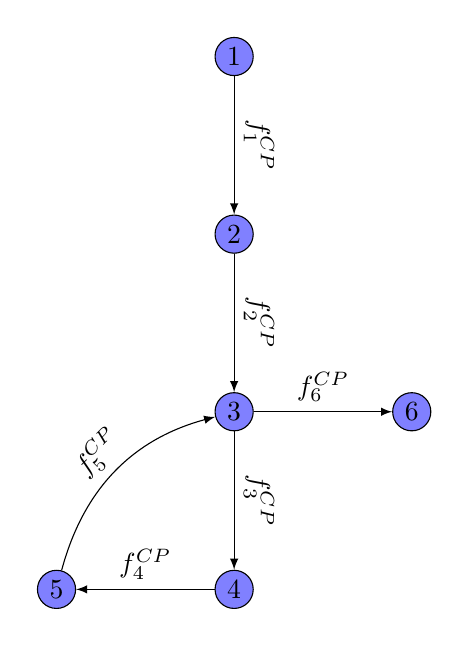
\begin{tikzpicture}[node distance = 2cm]
\matrix[row sep =5em,column sep=5em]{
 &\node(vert9)[state]{1}; &\\
 &\node(vert8)[state]{2}; &\\
 &\node(vert5)[state]{3}; &\node(vert2)[state]{6};\\
 \node(vert3)[state]{5}; &\node(vert4)[state]{4}; &\\
};
\draw [myarrow]  (vert9)  --  node[sloped, above]{$f_1^{CP}$} (vert8);
\draw [myarrow]  (vert8)  --  node[sloped, above]{$f_2^{CP}$} (vert5);
\draw [myarrow]  (vert5)  -- node[sloped,above]{$f_3^{CP}$}  (vert4);
\draw [myarrow]  (vert4)  --  node[sloped, above]{$f_4^{CP}$} (vert3);
\draw [myarrow]  (vert3) edge[bend left]  node[sloped, above]{$f_5^{CP}$} (vert5);
\draw [myarrow]  (vert5)  -- node[sloped,above]{$f_6^{CP}$}  (vert2);
\end{tikzpicture} 
\end{minipage} \hfill
\begin{minipage}[t]{.45\textwidth}
\begin{eqnarray*} 
\hat{\sigma}_1 & = & \{x\rightarrow\top, y\rightarrow\top,z\rightarrow\top\}\\
\hat{\sigma}_2 & = & f_1^{CP} (\hat{\sigma}_1) \\ 
\hat{\sigma}_3 & =& f_2^{CP} (\hat{\sigma}_2) \sqcup  f_5^{CP} (\hat{\sigma}_5)\\
\hat{\sigma}_4 & = & f_3^{CP} (\hat{\sigma}_3) = \hat{\sigma}_3 \\ 
\hat{\sigma}_5 & = & f_4^{CP} (\hat{\sigma}_4) \\ 
\hat{\sigma}_6 & = & f_6^{CP} (\hat{\sigma}_3) = \hat{\sigma}_3 
\end{eqnarray*}

\vspace{\fill}

~
\end{minipage}
\end{document}

